% Peekaboo-VL report: 05_method. Included from ../peekaboo_report.tex.
\section{Method}
\label{sec:method}

Fig.~\ref{fig:system} shows the whole pipeline. We explain it in the order
in which a question goes through it.


\subsection{Step 1: decode each clip once}
Decoding video is the slowest part of reading it, and each clip is used by
about 15 questions. So each clip is decoded once into a cache of 64 evenly
spaced frames. For all 1,047 clips this takes under a minute and about
7\,GB of disk; after that, loading a clip's frames is a plain file read. Together
with the frames we store the clip's frame rate and the exact frame numbers
we took. From these, the true time of every frame is known. The final
model takes 32 of the 64 frames (our first runs used 16). Each frame comes
from one of 32 equal time segments, a standard choice from action
recognition~\cite{wang2016tsn}. A ``phase'' setting decides where inside
its segment a frame is taken. At test time we take the centre. During
training we draw a new random phase for every question, so the model sees
many different sets of timestamps for the same clip. A model trained on one
fixed set of frames gets worse when the frames shift
(Sec.~\ref{sec:ablation}); random phases remove that weakness, and they act
as a small data augmentation as well.

\subsection{Step 2: two processor defaults that silently hurt}
Two default settings in the Qwen3.5 video processor would have hurt us.
Neither raises an error or a warning; we only found them by reading the
prompt the processor actually builds.

\emph{Image size.} The processor has a pixel budget
(\texttt{size.longest\_edge}, default 786,432 pixels). This budget covers
\emph{all} frames together, not each frame. With 32 frames, it would shrink
each 640$\times$360 frame to about 208$\times$117 pixels, where a car is
just a few pixels. We scale the budget with the number of frames, so each
frame stays at 640$\times$352. This gives 220 visual tokens for each pair
of frames, about 3,500 for the 32 frames of a clip.

\emph{Timestamps.} The processor computes frame times from video metadata.
When frames are given without that metadata, it assumes 24 frames per
second, so the times written in the prompt are wrong. Our cache passes the
true frame rate and frame numbers. We checked the final prompt for a
25\,fps, 15\,s clip and it contains the correct
\texttt{<1.9/5.6/9.3/13.1 seconds>} labels.

\subsection{Step 3: measure the camera motion}
For each pair of neighbouring sampled frames we do the following
(Fig.~\ref{fig:probe}).
\begin{enumerate}
\item Find a few hundred distinctive points (ORB
keypoints~\cite{rublee2011orb}) in both frames, such as road markings and
roof corners.
\item Match points between the two frames. A ``ratio test'' throws away
matches that are not clearly better than the second-best choice.
\item Fit one transform that explains most matches: a shift, a zoom and a
rotation (a ``similarity'' transform with four numbers). RANSAC
\cite{fischler1981ransac} handles the outliers: it tries many small random
sets of matches and keeps the transform that agrees with the most of them.
Matches on moving cars do not agree with the ground, so they are ignored.
\item Turn the four numbers into a label. The camera moves opposite to the
scene: if the ground slides to the left, the camera is panning right. A
camera tilted forward and flying forward sees the ground slide down and
grow larger. Rotation means the camera turns. Small numbers mean the camera
is still.
\end{enumerate}
We then join neighbouring steps with the same label into timed segments,
and fold segments shorter than 0.8\,s into a neighbour. The whole probe
takes a few milliseconds per frame pair on one CPU core; all 1,047 clips
take under a minute.

Why not a learned motion model? Because this one needs no training, no GPU
time and no labels, and its output is a sentence we can read and check.
When it is wrong, we can see why (Sec.~\ref{sec:results} shows where it
fails).

\begin{figure}[t]
\centering
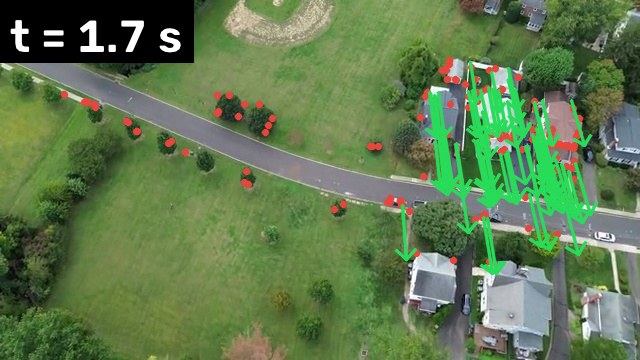
\includegraphics[width=0.92\columnwidth]{figures/probe_tracks.jpg}
\caption{The motion probe between two sampled frames of the clip in
Fig.~\ref{fig:sample}. 304 of 450 point matches agree with one transform
(green, 80 shown at random). They all stream downward, which is what
forward flight looks like. Red dots are rejected matches, here on trees
whose leaves all look alike.}
\label{fig:probe}
\end{figure}

\subsection{Step 4: write the motion in the answers' words}
The first version of the hint described what happens \emph{in the image}:
``pans toward the top of the frame, fast and zooms in (descending)''.
Section~\ref{sec:cue} shows that this wording confused the model. The final
version uses the words of ReVA's camera-motion answers: \emph{moving
forward / backward}, \emph{panning left / right}, \emph{rotating},
\emph{stationary}, with a speed word and a short summary at the end, for
example:

\smallskip
\noindent\fbox{\parbox{0.95\columnwidth}{\footnotesize\ttfamily
Camera motion: 0.1-5.9s moving forward quickly while rotating clockwise.
Mostly moving forward (100\% of the clip).}}
\smallskip

\subsection{Step 4b: a second hint, counts from a detector}
\label{sec:counts}
The camera hint says how the \emph{camera} moves, not how many objects are
in the scene. Video models are known to undercount small, dense objects, and
``Object \& Land Cover'' is one of ReVA's largest tasks. We therefore add a
second hint produced by a VisDrone-trained detector (YOLO11x), the only
learned component in the pipeline besides the model itself. The detector
runs on the first, middle and last of the clip's cached frames, and its
counts are merged into the words the questions use (``person'', ``car'',
``truck'') and written as one sentence:

\smallskip
\noindent\fbox{\parbox{0.95\columnwidth}{\footnotesize\ttfamily
Detector counts: 0.0s car 23, pedestrian 4, truck 2; 3.0s car 19; 5.9s car
31, truck 3.}}
\smallskip

ReVA's counting answers are ranges (``10--20''), so a detector error of
about 20\% usually still lands in the correct range. The counts are
computed once for all 1,047 clips and stored next to the motion hints, so
training and testing add no detector cost. We built the hint for every
clip but did not get to evaluate it within our compute budget, so the
final model does not use it.

\subsection{Step 4c: a clock drawn on the frames of timing questions}
\label{sec:timebar}
The timestamps in the prompt tell the model \emph{when} each frame was
taken, but only as text next to the frames. Temporal Grounding questions ask
exactly this (``At what time does the red car first appear?''), and they
are our weakest task. Following VTimeCoT~\cite{zhang2025vtimecot}, we also
\emph{draw} the time on the frames: a dark strip along the bottom edge, a
red bar that fills from left to right as the clip plays, and the frame's
time in seconds (``3.5s''). The model can then read the time from the image
itself.

We draw the bar only for Temporal Grounding questions. Drawing it on every
question helped timing questions but cost object questions, because the
strip covers the bottom 16 pixels of the frame, where small cars and people
often are. The bar is drawn the same way in training and in testing, so the
model learns to use it. Tested on a model that was trained without it, the
bar already raised Temporal Grounding by 0.9 points on dev.

\subsection{Step 5: build the prompt}
The model receives one user message: the 32 frames with their timestamps
(with the drawn clock for Temporal Grounding questions), then the hint line,
the question, the four options and a fixed instruction.
Qwen3.5 can ``think'' in
writing before answering; we switch this off, so the answer letter comes
right after the start of the model's reply.

\subsection{Step 6: score the four letters}
At the answer position we read the model's scores (logits) for the tokens
A, B, C and D and treat them as the scores of four classes. To save memory,
we compute scores only for that one position. During training, the loss is
the usual cross-entropy over these four scores. In other words, we train
the model to put high probability on the correct letter, and we ignore all
other words. There is no text generation and no answer parsing.

We chose this over generating an answer for three reasons. It never fails
to produce a valid letter. It gives four scores per question, which the
later steps (letter debiasing, mixing in a prior, combining models) need.
And it is cheap: computing scores only for the last position avoids
building the full 250k-word output layer for every token. Scoring takes
0.63\,s per question on the A40 at 16 frames and about 1.4\,s at 32 frames
(Step~7b makes this faster).

\subsection{Step 7: fine-tune with LoRA}
We attach LoRA adapters~\cite{hu2022lora} (rank $r{=}64$, scale
$\alpha{=}128$, dropout 0.05) to every linear layer of the language model.
This covers the attention layers, the Gated DeltaNet layers and the
feed-forward layers. We also attach them to the small ``merger'' that
connects the vision part to the language part. The vision encoder itself
stays frozen. In total, 161.6M of 9.57B parameters are trained (1.69\%).
The adapter file is about 620\,MB, so keeping many experiments around is
cheap, and training at 32 frames fits in 28\,GB of the A40's 46\,GB.

The final model trains on all 14,068 fit questions for one pass, with one
question per sequence. A second pass did not help: with branching
(Step~7b) and the learning rate decayed over two passes, the two-pass model
ends at 82.96\% test-weighted dev, against 83.04\% for one pass. A faster recipe packs eight questions about one clip
into one sequence (Sec.~\ref{sec:packing}). Packing costs accuracy, and we
now know why: each later question in the sequence can see the correct
answers to the earlier ones. The model therefore trains on a prompt it never
sees at test time, and with packing, more training data did not help.
Step~7b gives the speed of packing without this leak.

Every time a training question is used, we shuffle its four options into a
new random order. The correct answer is therefore equally likely to be A,
B, C or D, and the model cannot learn to prefer a letter.
Table~\ref{tab:setup} lists all settings of the main run.

\begin{table}[t]
\centering
\caption{Training and test settings of the final model (H20).}
\label{tab:setup}
\footnotesize
\begin{tabular}{@{}ll@{}}
\toprule
Base model & Qwen3.5-9B, bf16, SDPA attention \\
Video input & 32 frames, 640$\times$352, true timestamps \\
Frame sampling & random phase per question (train), centre (test) \\
Hints & camera motion, in answer words; \\
 & drawn clock on Temporal Grounding frames \\
Adapter & LoRA $r{=}64$, $\alpha{=}128$, LM linears + merger \\
Data & all 14,068 fit questions, one per sequence \\
Optimizer & AdamW, lr $10^{-4}$, 3\% warm-up, cosine decay \\
Batch & 1 $\times$ 16 accumulation, 880 steps (1 pass), clip 1.0 \\
Training time & 17\,h (about 70\,s per 16-question step) \\
Hardware & 1$\times$ NVIDIA A40 (46\,GB), 28\,GB used \\
Speed & 4.3\,s per training question \\
Decoding & PriDe~\cite{zheng2024pride} (5\% subset) or plain \\
\bottomrule
\end{tabular}
\end{table}

\subsection{Step 7b: one video pass for many questions, without leaks}
\label{sec:branch}
Each clip has about 15 questions, and the video makes up almost all of the
prompt (about 3,500 of 3,700 tokens). Scoring the questions one by one
therefore processes the same video 15 times. We split each prompt into a
\emph{prefix} shared by all questions about the clip (the video and the hint)
and a short \emph{suffix} per question (the question, the options and the
start of the answer). The prefix runs through the model once, and every
suffix then continues from it on its own branch:
\begin{itemize}
\item In the full-attention layers, each suffix attends to the prefix and to
its own earlier tokens, never to another suffix.
\item In the Gated DeltaNet layers, which keep a running state instead of
attending, each suffix starts from the state the prefix ends in (and from
the last few inputs of the layer's short convolution).
\end{itemize}
Every question therefore sees exactly the prompt it would see alone, so
nothing leaks between questions, and during training the gradients of all
branches add up in the shared prefix. We checked this against scoring the
questions one at a time on Qwen3.5-0.8B in 32-bit floats: the letter scores
agree to $10^{-4}$ and the adapter gradients to a relative $6\times10^{-5}$.
In 16-bit floats the scores move by rounding only. Scoring eight questions
per video pass was 3.7 times faster in our test, and the same split makes
training about as fast as packing. Questions with and without the drawn clock
see different frames, so they go into separate groups.

\subsection{Step 7c: two more training signals (being tested)}
\label{sec:extra-losses}
Both signals change only the training loss; the test prompt stays the same.

\emph{The clip played backwards.} Video models often give the same answer
when the frames are shuffled or reversed, which means they answer from what
is in the frames, not from their order~\cite{kang2026bpo}. For questions
whose answer must change when time runs backwards, we also show the model
the reversed clip and push it away from the original answer. These are
Temporal Grounding questions about a moment (``when does the bus first
appear''), Change Detection questions about a direction or a change, and
camera-motion questions (``moving forward''). Questions whose answer stays
the same, such as durations, a stationary camera or the viewing angle, are
left out by simple text rules; about 16\% of the fit questions qualify. The
reversed clip keeps its timestamps and clock running forward, and it gets
no motion hint, because the hint describes the original direction. With
$p_{\text{rev}}(y)$ the probability of the original answer $y$ on the
reversed clip, the loss becomes
\[
\mathcal{L} = \mathrm{CE} + \lambda_{\text{rev}}\,
\bigl(-\log\,(1 - p_{\text{rev}}(y))\bigr),\qquad \lambda_{\text{rev}} = 0.5 .
\]
The extra term only says ``not this answer''; it does not name a new one,
and it fades once the original answer is unlikely. Before spending a run on
it, we test whether the trained model already changes its answers on
reversed clips; if it does, this signal has little to teach.

\emph{The clip's facts as plain text.} The test set asks new questions about
clips the model has already trained on. In language models, facts learned
in a single format are often not recalled when the question is asked in a
new way; training on the same facts in two formats at once fixes much of
this~\cite{zhang2025factrecall}. Our training uses one format only: pick a
letter for four given options. So each group of questions about a clip gets
one extra branch (Step~7b) in which the model writes out that clip's
training questions with their answers as plain text, without options or
letters (``Q: When does the red car first appear? A: At 3.5 seconds''). The
pairs are shuffled every time and capped at 24. The loss adds
$\lambda_{\text{fact}} = 0.3$ times the mean word-level cross-entropy of this
text. Because the text branch is a separate branch, the letter questions
never see it; we checked that their scores are identical with and without
it. Dev questions never appear in the text.

\emph{Outcome.} The reversed-clip check ran first, on the final model's
dev answers: on the 375 questions whose answer should change, the model
kept its answer on the reversed clip 68.3\% of the time, against 88.0\% on
266 control questions whose answer should not change. The model already
uses frame order where it matters, so by our pre-registered rule (a gap
below 0.15 would justify the run; it is 0.197) we did not train with this
signal. The fact-text signal was built and checked but not trained within
our budget.

\subsection{Step 8 (optional): remove letter bias and mix in a text prior}
\label{sec:blind}
\emph{Letter bias.} PriDe~\cite{zheng2024pride} estimates how much the
model prefers each letter by scoring a small part of the test set with the
options rotated. It then divides this preference out of every score. It
needs no correct answers.

\emph{Blind prior.} We also train a small text-only scorer that never sees
the video. For each option it computes 50 simple features: how long the
option is compared with the others, how often similar answer texts were
correct in training for this task, how many words it shares with the
question, whether it is the largest or smallest number among the options,
and a few task-specific copies of the strongest features. A logistic model
over the four options learns how to weigh these features. It trains in
seconds. At test time we can combine it with the video model as
$\log p = \log p_{\text{VLM}} + \alpha \log p_{\text{blind}}$, where
$\alpha$ controls how much we trust the blind scorer. We choose $\alpha$ on
dev with cross-validation, with the folds split by clip so no clip is in
both halves.

\emph{Plain decoding.} Because the options are shuffled in training, the
fine-tuned model has almost no letter preference left, so PriDe has little
to correct. We therefore also tried plain scores: one pass with the official
option order and no correction. On dev the plain scores looked slightly
better, but on the test set PriDe won (83.55\% vs.\ 83.25\%). The plain
answers lean slightly towards ``A'' (26.9\% of answers), which is exactly
what PriDe removes. We keep PriDe. A dev difference below about one point
between two decodings of the same model is not a reliable guide.

\emph{Averaging over frame phases.} Shifting all frames by half a segment
changes about one answer in five on video benchmarks while leaving accuracy
unchanged~\cite{zhu2026phase}. A model trained with random phases (Step~1)
can be scored at several phases, for example 0.17, 0.5 and 0.83, and its
answer probabilities averaged. This removes the dependence on one phase at
the cost of one scoring pass per phase. We implemented it but did not
evaluate it; the submitted system scores the centre phase only.
